In this section we present our predictions for the population of detectable LISA sources for our fiducial model. In total we expect, on average, $124$ detections in a 4-year LISA mission, of which $\BHBHFourYear{}$, $\BHNSFourYear{}$ and $\NSNSFourYear{}$ are BHBHs, BHNSs and NSNSs respectively, based on our fiducial simulations. In the remainder of this section, we discuss where the sources are expected relative to LISA's sensitivity curve (Sec.~\ref{sec:dcos_on_sc}), their properties (Sec.~\ref{sec:fiducial_distributions}), their locations in the Milky Way (Sec.~\ref{sec:mw_detectable_distribution}), their formation channels (Sec.~\ref{sec:progenitors_and_formation}) and finally we discuss the expected SNR and how accurately we expect that the parameters can be measured (Sec.~\ref{sec:measurement_uncertainties}). Note that all results shown in this section are based on our fiducial simulations. A discussion of the impact of variations in the physics assumptions is provided in Sec.~\ref{sec:variations}.

\subsection{The LISA sensitivity curve and the population of detectable sources}\label{sec:dcos_on_sc}
\begin{figure*}[p]
    \centering
    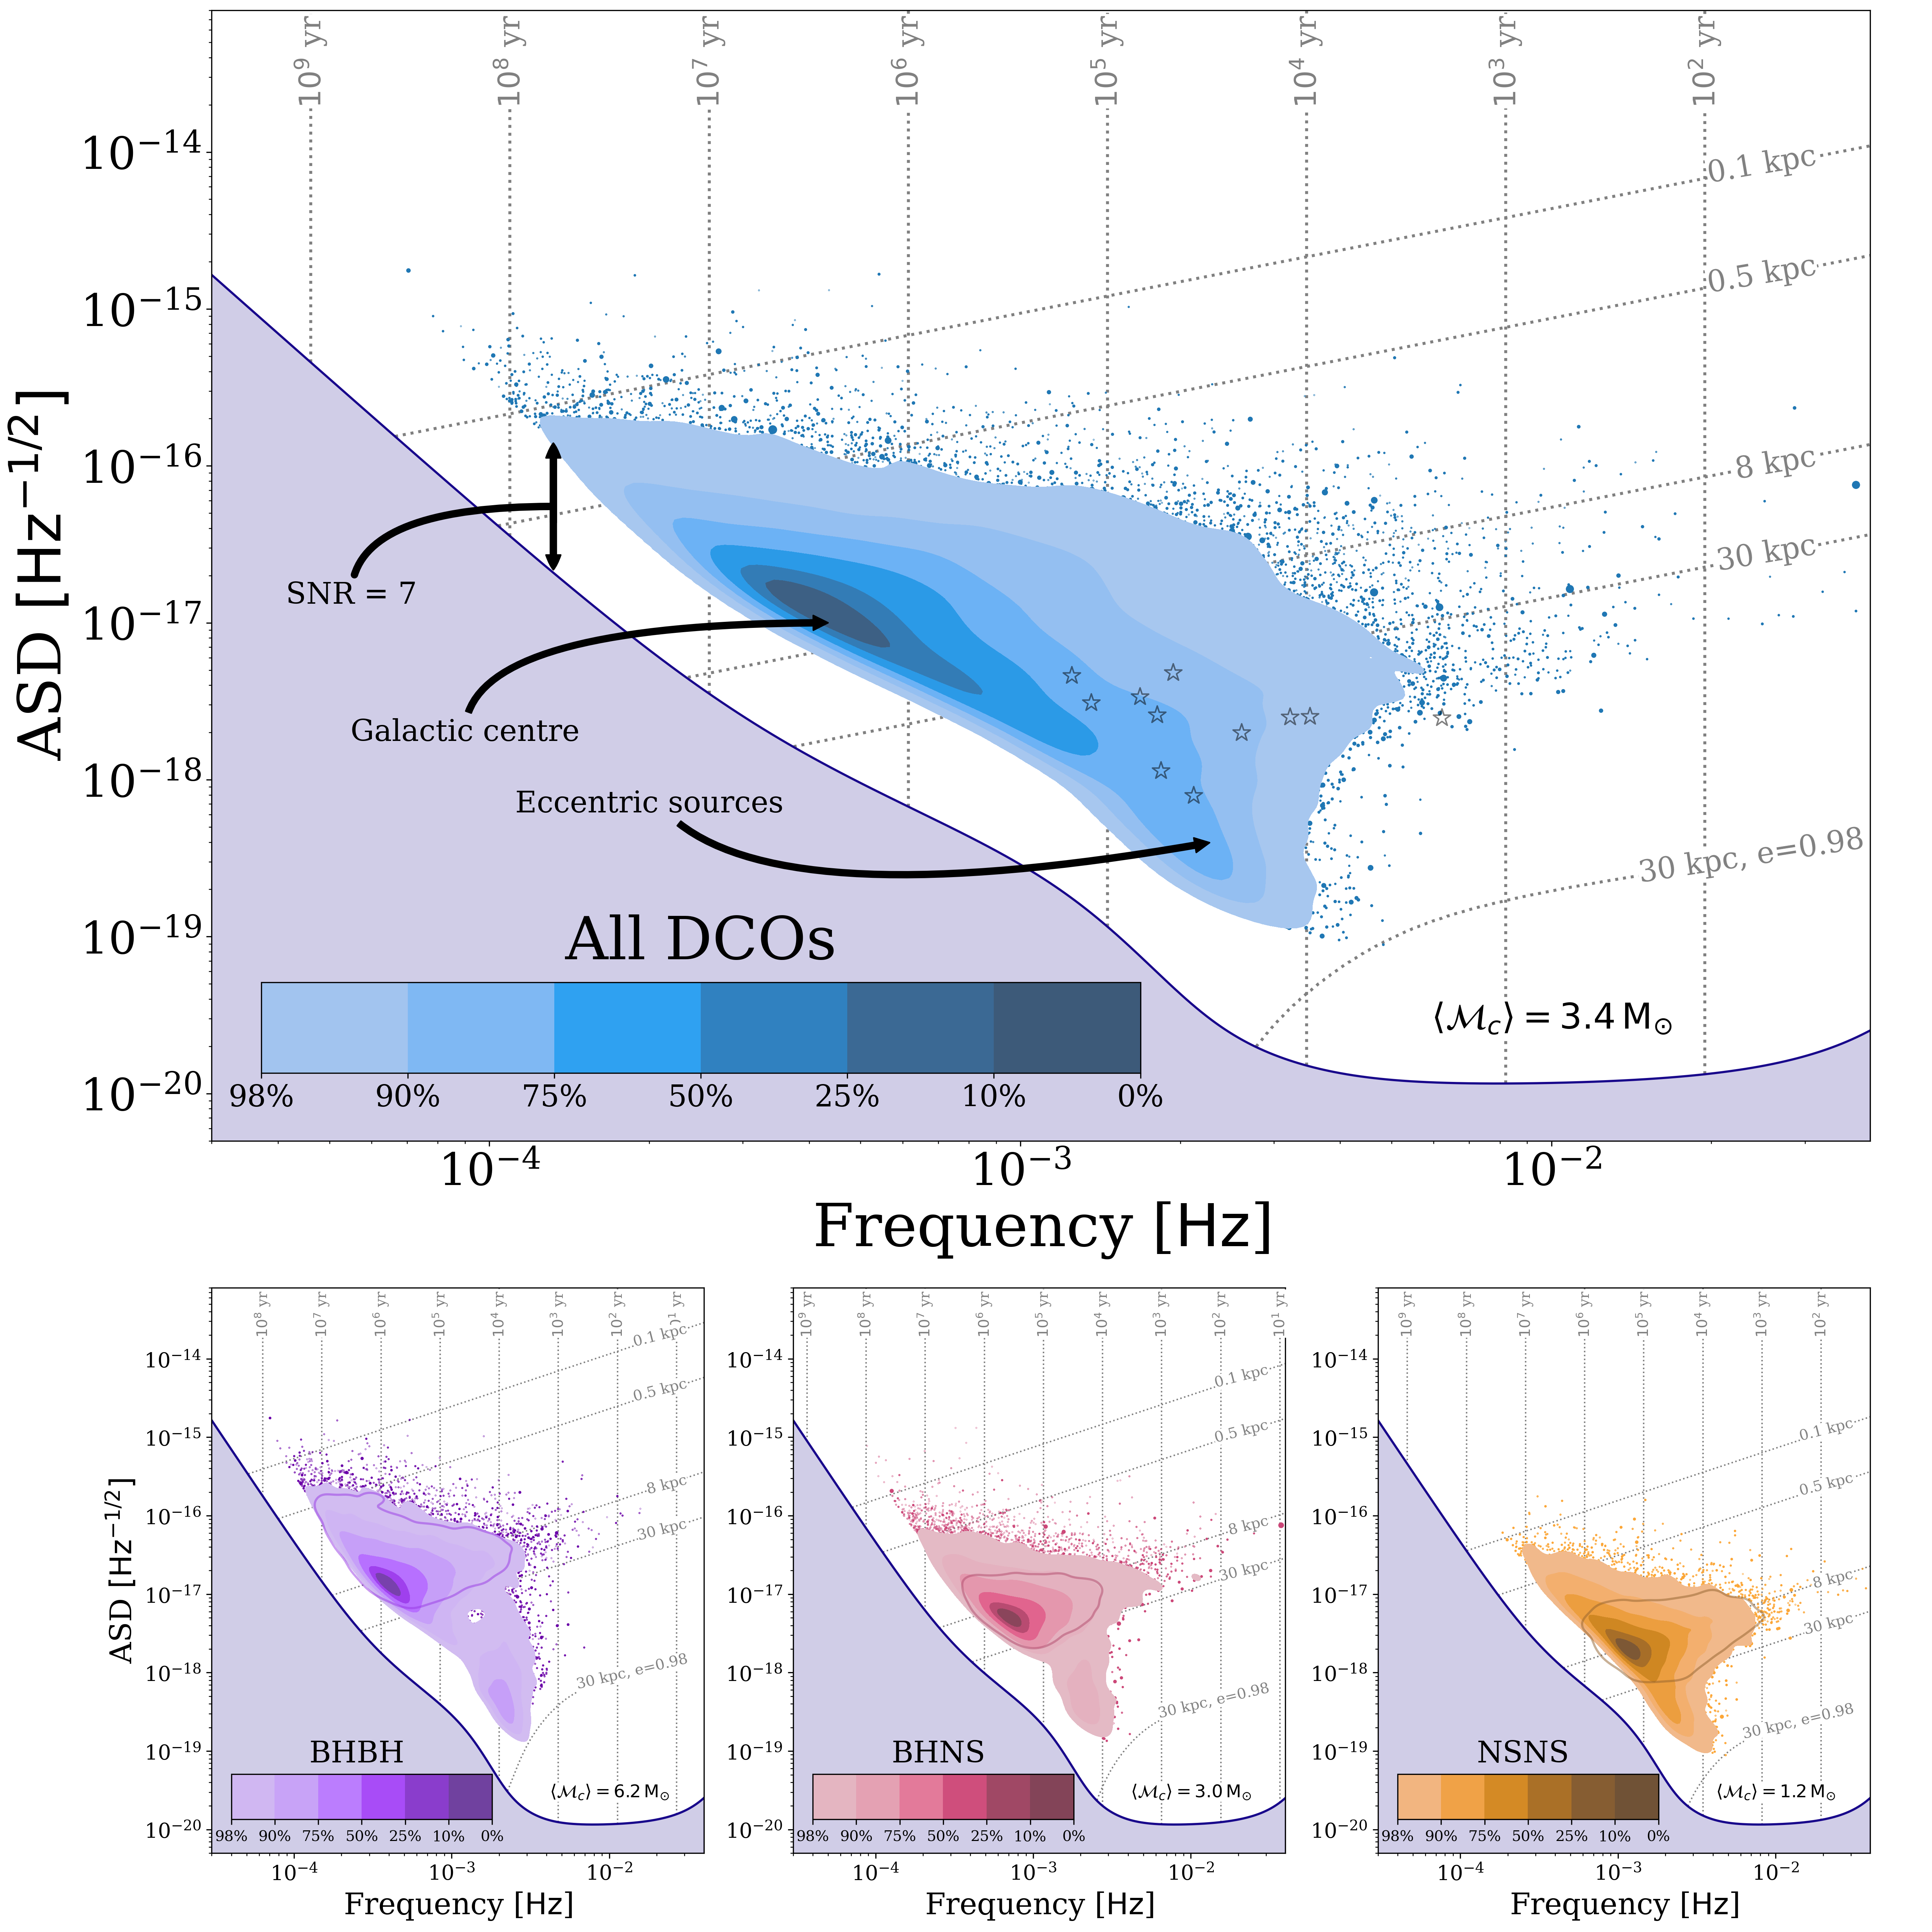
\includegraphics[width=\textwidth]{fig2_dcos_on_sc.png}
    \caption{The LISA sensitivity curve is shown together with the density distribution of the characteristic strain and the dominant frequency for all detectable sources in our simulations (top) and separated by type (bottom). Contours show the percentage of the population enclosed. The remaining 2\% of the population is shown as dots with a size that scales with the sampling weight. To guide the interpretation, we show reference lines marking where a circular binary would reside for a given distance (diagonal line) and remaining inspiral time (vertical lines), assuming an average chirp mass $\avg{\mathcal{M}_c}$, orientation and sky location. The coloured lines in the bottom panels show a contour that encloses 90\% of the population that is circular. LISA verification binaries are overplotted in the top panel (star symbols).  See also Fig.~\ref{fig:dcos_on_sc_ecc_col} and Sec.~\ref{sec:dcos_on_sc} for a discussion. \href{https://github.com/TomWagg/detecting-DCOs-in-LISA/blob/main/paper/figures/fig2_dcos_on_sc.png}{\faFileImage} \href{https://github.com/TomWagg/detecting-DCOs-in-LISA/blob/main/paper/figure_notebooks/sensitivity_curve.ipynb}{\faBook}.}
    \label{fig:dcos_on_sc}
\end{figure*}
We show the expected LISA sensitivity curve \citep{Robson+2019} in Fig.~\ref{fig:dcos_on_sc}, which includes the confusion noise arising from the Galactic WDWD population, and overplot our predictions for the distribution of detectable sources. Eccentric systems emit gravitational waves in multiple harmonic frequencies ($n f_{\rm orb}$, with $n = 2, 3, \dots $). We choose to plot them at the $x$-coordinate that corresponds to the frequency of the harmonic that individually accumulates the largest SNR. For circular systems, the $x$-coordinate simply corresponds to $2 f_{\rm orb}$. The $y$-coordinate indicates the strength of the signal (or to be more precise, the amplitude spectral density, ASD), including the contribution from \textit{all} harmonics.

For reference, we show dotted lines to indicate where a hypothetical binary system would reside assuming a given distance from earth (diagonal lines) and a fixed remaining inspiral time (vertical lines). For each line we assume the binary is circular and has a chirp mass equal to the average of the sample ($\avg{\mathcal{M}_c}$, annotated in each panel). We also overplot the LISA verification binaries (star symbols, \citealt{Kupfer+2018}).

\vspace{1em}

We observe several features in Fig.~\ref{fig:dcos_on_sc} that are worth discussing and explaining. We note that some of these have also been described in earlier studies (see Sec.~\ref{sec:compare_studies}). Firstly, we note the empty band that separates the LISA sensitivity curve and the detectable population. This is the result of the criteria for detection where we require $\rm{SNR} > 7$.

We further note that the detectable population is concentrated on the left side of LISA's sensitivity window. The peak is located at a frequency of about $0.4 \unit{mHz}$, which is much lower than the frequency where LISA will be most sensitive (about $10 \unit{mHz}$). This can be understood from the acceleration of inspiraling DCOs as they evolve towards higher frequencies. DCOs typically form with wide orbits (low frequencies) that would not be detectable yet. Their orbits shrink as they lose angular momentum in the form of gravitational waves leading to an increase of their orbital frequency until they become detectable. These systems are increasingly rare because they evolve faster and faster towards higher frequency as the inspiral accelerates, even though the signal emitted by a more compact binary is stronger \citep{Peters+1964}. The vertical grid lines show these rapidly decreasing inspiral times at increasing frequencies. Most of the population is thus expected to reside at low frequencies.

In the lower three panels, we show the contributions of the different types of sources. Comparing them, one can observe the shift in the frequency at which the peak is located, at $0.3 \unit{mHz}$, $0.7 \unit{mHz}$ and $1 \unit{mHz}$ for BHBH, BHNS and NSNS systems respectively. This is a result of the difference in chirp mass. A higher mass system can emit at lower frequency and still produce the minimum SNR needed for detection. We note that this effect can be used to distinguish the heavier DCOs that we discuss in this work from WDWD systems, at least probabilistically (see Sec.~\ref{sec:WDWD_distinguish}). In the same way, this also explains the offset in frequency between the population of sources we predict and the LISA verification binaries.

Inspecting the dotted reference lines, we note that the peak of the density distribution of observable sources coincides with the location expected for circular systems at $8 \unit{kpc}$, which is the distance to the centre of the Milky Way. As can be seen best in the lower panels, the reference lines for $0.1$ and $30 \unit{kpc}$ enclose the majority of systems, as expected given the dimensions of the Milky Way.

There is a distinct subpopulation of binaries, most clearly visible in the lower panels as an offshoot that extends downwards to ASDs of $10^{-19} \unit{Hz}^{-1/2}$, especially around $2 \unit{mHz}$. This offshoot is almost uniquely composed of eccentric binaries, as can be seen in Fig.~\ref{fig:dcos_on_sc_ecc_col}, which shows a similar figure but colouring individual systems by their eccentricity. This can also be seen, albeit indirectly, from the contour lines shown in the bottom panels of Fig.~\ref{fig:dcos_on_sc}, which encompass 90\% of the \textit{circular} sources in each population. This contour does not include the offshoot. We conclude that eccentric sources occupy a very different region in this diagram.

\subsection{Properties of the detectable systems}\label{sec:fiducial_distributions}
In Fig.~\ref{fig:fiducial_pdf_distributions}, we show the 1D distribution of several individual parameters of the population of detectable binaries together with the 1- and 2-$\sigma$ uncertainties obtained via bootstrapping. These uncertainties represent the fluctuations in our results over different random instances of the Milky Way. The distributions shown here are approximated by kernel density estimators, corrected for edge effects by mirroring the sample \citep{Schuster+1985}.

\paragraph{Orbital Frequency} The orbital frequency distributions for BHBHs, BHNSs and NSNSs (Fig.~\ref{fig:fiducial_pdf_distributions}a) peak at progressively increasing frequencies. As mentioned in Sec.~\ref{sec:dcos_on_sc}, this is because a higher mass DCO at the same distance and eccentricity requires a lower frequency to produce the same signal-to-noise ratio and thus be detected. The distributions appear nearly symmetric, but closer inspections shows that the left hand side is more populated, which can be seen most clearly in the curve for the BHBHs. This is due to the contribution of highly eccentric binaries, which are most abundant in the BHBH population. These systems are still detectable by LISA, despite their low orbital frequency, as the high eccentricity means that the majority of the GW signal is emitted at higher harmonics, where LISA is more sensitive.

\begin{figure*}[t]
    \centering
    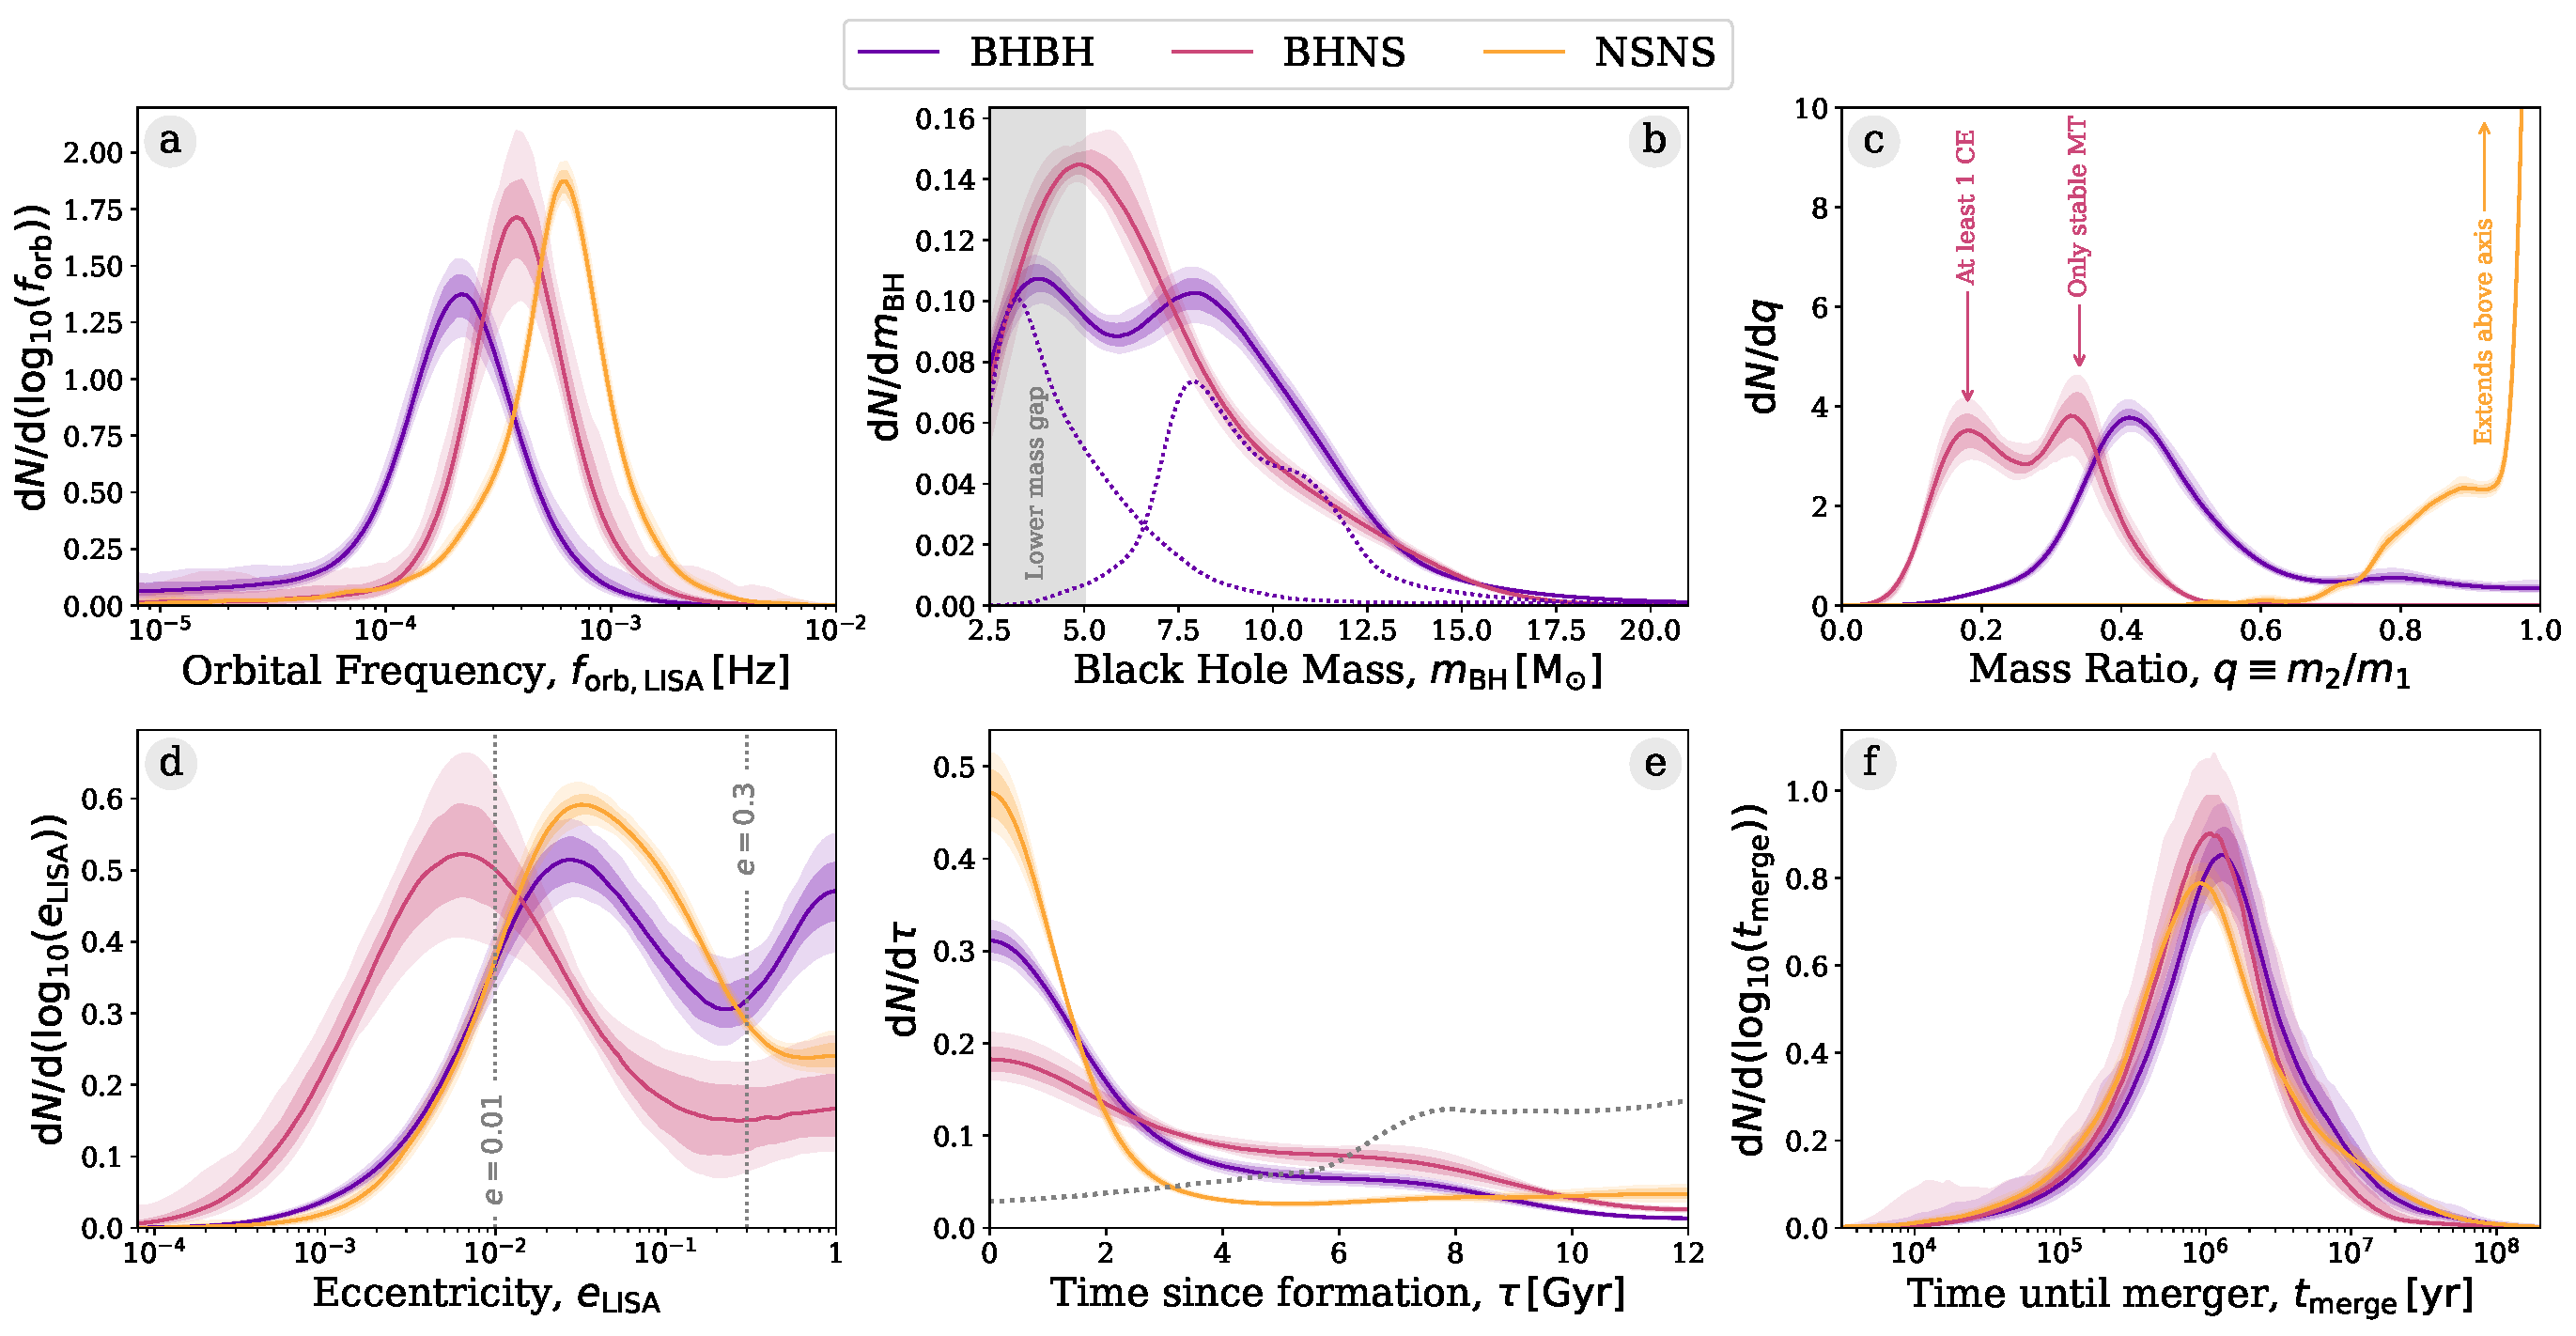
\includegraphics[width=\textwidth]{fig3_detectable_properties_4yr.pdf}
    \caption{Properties of detectable systems for a 4-year LISA mission in our fiducial model. Each panel shows a kernel density estimator for a single property, coloured by DCO type. Each curve has been individually normalised. The shaded areas show the 1- and 2-$\sigma$ sampling uncertainties (obtained via bootstrapping). The dotted lines in panel b show the individual primary and secondary mass distributions. The dotted line in panel e shows the star formation history we have assumed in our Milky Way model. See Sec.~\ref{sec:fiducial_distributions} for a discussion. \href{https://github.com/TomWagg/detecting-DCOs-in-LISA/blob/main/paper/figures/fig3_detectable_properties_4yr.pdf}{\faFileImage} \href{https://github.com/TomWagg/detecting-DCOs-in-LISA/blob/main/paper/figure_notebooks/fiducial.ipynb}{\faBook}.}
    \label{fig:fiducial_pdf_distributions}
\end{figure*}

\paragraph{Black Hole Mass}
In Fig.~\ref{fig:fiducial_pdf_distributions}b, we show the distribution masses of individual black holes that are part of BHNS and BHBH systems. 
The distribution for BHBH shows a bimodality. This results from the two contributions of the more and less massive BHs in BHBH systems, which peak at around $8 \unit{M_{\odot}}$ and $3.5 \unit{M_{\odot}}$ respectively as shown by the dotted lines (see also our discussion of the mass ratios below).

For both the BHBHs and BHNSs, we see that the black hole mass distribution favours low masses. About $90\%$ of BHs have masses below $11 \unit{M_{\odot}}$, in our fiducial simulations shown here. This is in stark contrast with observations from ground-based GW detectors, where heavy BHs with masses of about $30\unit{M_{\odot}}$ and higher have been common. There are two main reasons for this discrepancy. First, the population of BHs in the Milky Way (and, in particular, those detectable by LISA due to their recent formation times, see Fig.~\ref{fig:fiducial_pdf_distributions}e) primarily come from progenitors that formed from high metallicity gas according to our simulations. Stellar winds are stronger at high metallicity leading to increased mass loss. This affects the mass of the most massive black holes that can be formed \citep{Belczynski+2010}. Secondly, ground-based detectors are strongly biased towards high mass systems, since they can be detected out to larger distances and thus a greater volume is probed. In contrast, LISA has no such bias and is, in principle, sensitive to inspiraling BHBHs throughout the entire Milky Way regardless of their mass, as long as we catch them when they are emitting in the LISA band. For this reason, LISA is more likely to detect the more common lower mass BHBHs. 

We also note that our BH mass distribution extends down below $5\unit{M_{\odot}}$ to $2.5 \unit{M_{\odot}}$ which is our fiducial maximum neutron star mass. The BHs in this simulation fill the so-called ``lower mass gap'' marked as a grey band \citep{Ozel+2010,Farr+2011}, see also \citet{Shao+2021} who recently also pointed this out. This prediction is sensitive to adopted model for fallback during the SN explosion as we discuss this further in Section~\ref{sec:lower_mass_gap}.

\paragraph{Mass Ratio} The mass ratio distributions for each DCO type are very distinct from one another, as can be seen in Fig.~\ref{fig:fiducial_pdf_distributions}c. The majority of NSNSs have a mass ratio close to unity, with $\NSNSqAbovePointEight{}$ of systems having $q > 0.8$, where $q \equiv m_2 / m_1$. The reason for the concentration around equal masses is that most NSs are formed either through electron-capture supernovae (ECSN) or from low mass stars in our simulations. We assume a remnant mass for any NS formed through ECSN of $1.26 \unit{M_{\odot}}$ (see Sec.~\ref{app:fiducial_physics}). The remnant mass prescription that we use assumes a fixed fallback mass for any star with a CO core mass less than $2.5 \unit{M_\odot}$, such that many NSs end up with an identical mass of $1.278 \unit{M_\odot}$ \citep[see][Eq.~19]{Fryer+2012}. This means that many NSs are formed with equal masses and hence we see a mass ratio distribution peaked around unity.

In contrast, only $\BHBHqAbovePointEight{}$ of detectable BHBHs are formed with $q > 0.8$ and the distribution peaks around $q = 0.4$. We find that the strong stellar winds in our (typically high-metallicity) progenitors are the reason behind this. 

BHBHs with unequal masses typically come from progenitors that also had more extreme mass ratios at birth ($90$ and $30\unit{M_{\odot}}$ are typical for the progenitors of detectable BHBH systems in our simulations). The primary in such systems experiences strong mass loss by winds before filling its Roche lobe. This mostly happens during its early hydrogen-shell burning phase. The wind mainly reduces the mass of the envelope, but does not have a very strong effect on the core. By the time the primary fills its Roche lobe, it has become less massive and the mass ratio is closer to one. This favours stable mass transfer. The massive core of the primary star typically becomes the more massive BH. Accretion on the secondary star is limited and the secondary eventually provides the less massive black hole.

At the same time, stellar wind mass loss disfavours the formation of black holes with comparable masses. Such systems would have originated from progenitors that also started with comparable masses. The rather massive secondaries in these systems (especially after they accreted from the primary) experience very strong stellar wind mass loss due to LBV-like eruptions. This limits the amount by which they can expand \citep[e.g.][]{vanSon+2021}. At the same time, wind mass loss (and also stable and more conservative mas transfer in these systems) lead to widening of the orbit. Both effects, the reduced expansion and increased widening of the orbit, tend to prevent the secondaries from being able to fill their Roche lobe. This thus limits the number of systems that experience the reverse mass transfer or common-envelope phase needed shrink the orbits and make them tight enough to be detected as gravitational-wave sources.

We find that detectable BHNSs have even more unequal mass ratios. Moreover, the mass ratio distribution is bimodal, where the two peaks arise from two distinct formation scenarios. Around two thirds of detectable BHNSs experience at least one common-envelope event, whilst the last third are formed through only stable mass transfer. The first peak at $q = 0.18$ is from systems that experience at least one common-envelope phase and occurs at the expected mass ratio, which approximately follows the mean BH mass (${\sim}6.5 \unit{M_\odot}$) and NS mass (${\sim}1.2 \unit{M_\odot}$). Yet we also see a second peak at higher mass ratios around $q = 0.34$, which arises from the fraction of the population that underwent only stable mass transfer phases. The stability of mass transfer depends on the mass ratio, preferentially forming systems with more equal masses, i.e.\ at higher $q$.

\paragraph{Eccentricity} In Fig.~\ref{fig:fiducial_pdf_distributions}d we show the eccentricity distributions. We find that most systems (73\%) will have eccentricities larger than $0.01$ during the LISA mission, which should in principle be detectable according to \citet{Nishizawa+2016}. This means that we will potentially be able to use eccentricity to distinguish these sources from WDWDs, which are expected to have little to no eccentricity (see Sec.~\ref{sec:WDWD_distinguish}). We note that several previous studies assumed all systems to be circular when calculating the detection rates \citep[e.g.][]{Liu+2014, Lamberts+2018, Sesana+2020}. We discuss the impact of this assumption in Section~\ref{sec:compare_studies}.

For systems with eccentricities higher than $e\gtrsim0.3$, most gravitational wave energy is emitted in higher harmonics. Such systems are more rare, but we find them to be significant among the BHBH population, where they account for \BHBHHighlyEccentric{} of systems. Detectable BHBHs in our simulation (and, in particular, those that are eccentric) are primarily systems formed through the stable mass transfer channel (see Fig.~\ref{fig:formation_channels}). These systems are still relatively wide (compared to those formed through the CE channel) immediately prior to formation of the second BH, which makes them more easily affected by kicks. If the kick is oriented roughly in opposite direction to the orbital motion and has a velocity that is of similar magnitude as the orbital velocity, it will lead to the formation of a highly eccentric system. 

It is rare to get such a ``lucky kick'', but there are a few effects that favour this for BHBHs. The kicks of BHs are reduced by fallback and they are thus less likely to disrupt the system. Moreover, because of their higher masses, BHBHs can be observed already at lower orbital frequencies. This means that they have not had as much time to circularise and so still have significant eccentricity by the time of the LISA mission. Finally, LISA favours the detection of eccentric systems, if all other properties are held fixed. This is because the gravitational-wave emission is stronger (Eq.~\ref{eq:peters_f}) and the energy is emitted at higher frequencies \citep[Eq.~20]{Peters+1963} where LISA is more sensitive.

The lower abundance of highly eccentric systems among the NSNS and BHNS systems may seem counter-intuitive since neutron stars are lower mass and would be more strongly affected by natal kicks, which one may expect to lead to more eccentric systems. However, the majority of NSs in our simulations are formed through ECSN and USSN and for these types of supernovae we draw from a Maxwellian with $\sigma_{\rm rms}^{\rm 1D} = 30 \unit{km}{s^{-1}}$. Thus the kicks received by NSs in our simulations are often much smaller than for BHs.

\paragraph{Time since formation} 
In Fig.~\ref{fig:fiducial_pdf_distributions}e we show how long ago the LISA detectable DCOs formed. Star formation was highest at early times $6-12\unit{Gyr}$ ago, after which it declined. In contrast, the LISA detectable DCOs primarily formed in the relatively \textit{recent} history of our Milky Way, about $2 \unit{Gyr}$ ago. This reflects the fact that binaries in our simulation typically take about a Gyr to merge.

When comparing the distribution of formation times for the three different DCO types we see that NSNSs are most strongly concentrated at recent times, followed by BHBHs and then BHNSs. To understand this it is helpful to consider how the inspiral time scales with various parameters \citep{Peters+1964}
\begin{equation}
    t_{\rm inspiral} \propto \frac{a^4}{(m_1 + m_2)^{3}} \cdot \frac{q}{(1+q)^2} \cdot (1 - e^2)^{-7/2}.
\end{equation}
The inspiral time depends most strongly on the separation at DCO formation, $a$, and this is where the three types also differ most strongly (see Fig.~\ref{fig:dco_formation_properties}). The detectable NSNS systems have the tightest orbits at DCO formation. The median of the distribution of separations at DCO formation, $\langle a_{\rm DCO} \rangle_{\rm med}$, relate as 8:3:1 for detectable BHBH:BHNS:NSNS in our simulations. This results in increase of the inspiral time by a factor of about 4000:80:1. The total masses affect the inspiral time to the third power and this where the heavier BHBH systems are favoured. The median total masses differ by ratios of 6:4:1 for detectable BHBH:BHNS:NSNS in our simulations, impacting the inspiral times such that they are a factor of 200:60:1 shorter, partially counteracting the effect of the separations. The term depending on the mass ratio $q$ only varies by about 30\% for the mass ratio ranges considered here and so is not of interest. The eccentricity term is not of importance for mildly eccentric systems, $f(e_{\rm DCO} \le 0.3)  \le 1.4$ but of large importance for the very eccentric  $f(e_{\rm DCO} \ge 0.9) \ge 300$. The fraction of highly eccentric systems with $e_{\rm DCO}>0.9$ is 33\%, 16\%, and 8\% of for BHBH, BHNS and NSNS respectively, see also Fig.~\ref{fig:dco_formation_properties}. 

We conclude that the shorter median separations at DCO formation are the main reason why NSNS are most strongly peaked at short delay times. They are followed by BHBHs rather than BHNSs due to the high masses and substantial eccentricities of BHBHs.

\paragraph{Time until merger} Fig.~\ref{fig:fiducial_pdf_distributions}f shows the remaining time until merger for each of the DCO types at the start of LISA mission. The distributions are strikingly similar and peak with merger times of around a Myr.

The merger time is a function of the mass, frequency and eccentricity of the sources, such that more massive, higher frequency and more eccentric sources merge faster \citep[][Eq.~5.14]{Peters+1964}. So, despite the fact that each DCO type often has higher values in any one of these properties, the convolution of all three tends to negate the differences. For example, NSNSs have the highest orbital frequencies and are mildly eccentric whilst BHNSs have moderate orbital frequencies and are more circular. However, BHNSs are more massive in general and so the overall merger times are distributed very similarly for both DCO types.

\subsection{Distribution in the Milky Way}\label{sec:mw_detectable_distribution}
For our Milky way model we consider three different components, a low-\achem~(``thin'') disc, an older high-\achem~(``thick'') disc and a bulge/bar (see Sec.~\ref{sec:galaxy_synthesis}). In Table~\ref{tab:component_fractions} we summarise the number of detections originating from each of these components. Despite the fact that only $42.5\%$ of systems are formed in the low-\achem~disc, we find that $86\%$ of the detections originate from this component. This is because most detectable systems were formed relatively recently (see Fig.~\ref{fig:fiducial_pdf_distributions}e) and so the high-\achem~disc and bulge are effectively too old to contribute many detectable systems. Nevertheless, we do find a significant fraction of detectable systems originate in the high-\achem~disc and bulge, indicating that it is still important to include these components, as was ignored in some earlier works (see Sec.~\ref{sec:compare_studies}).

\begin{table}[tb]
    \centering
    \begin{tabular}{l|c|cccc}
        \hline
        \multirow{2}{*}{Component} & Formation & \multicolumn{4}{c}{Detectable} \\ \cline{2-6}
        & {\scriptsize All} & {\scriptsize All} & {\scriptsize BHBH} & {\scriptsize BHNS} & {\scriptsize NSNS} \\
        \hline
        Low-$\alpha$ disc & 42.5\% & 86\% & 89\% & 82\% & 85\%\\
        High-$\alpha$ disc & 42.5\% & 6\% & 5\% & 8\% & 12\%\\
        Bulge/bar & 15.0\% & 8\% & 6\% & 10\% & 3\%\\
    \end{tabular}
    \caption{Percentage of systems in each Galactic component.}
    \label{tab:component_fractions}
\end{table}
\begin{figure}[tb]
    \centering
    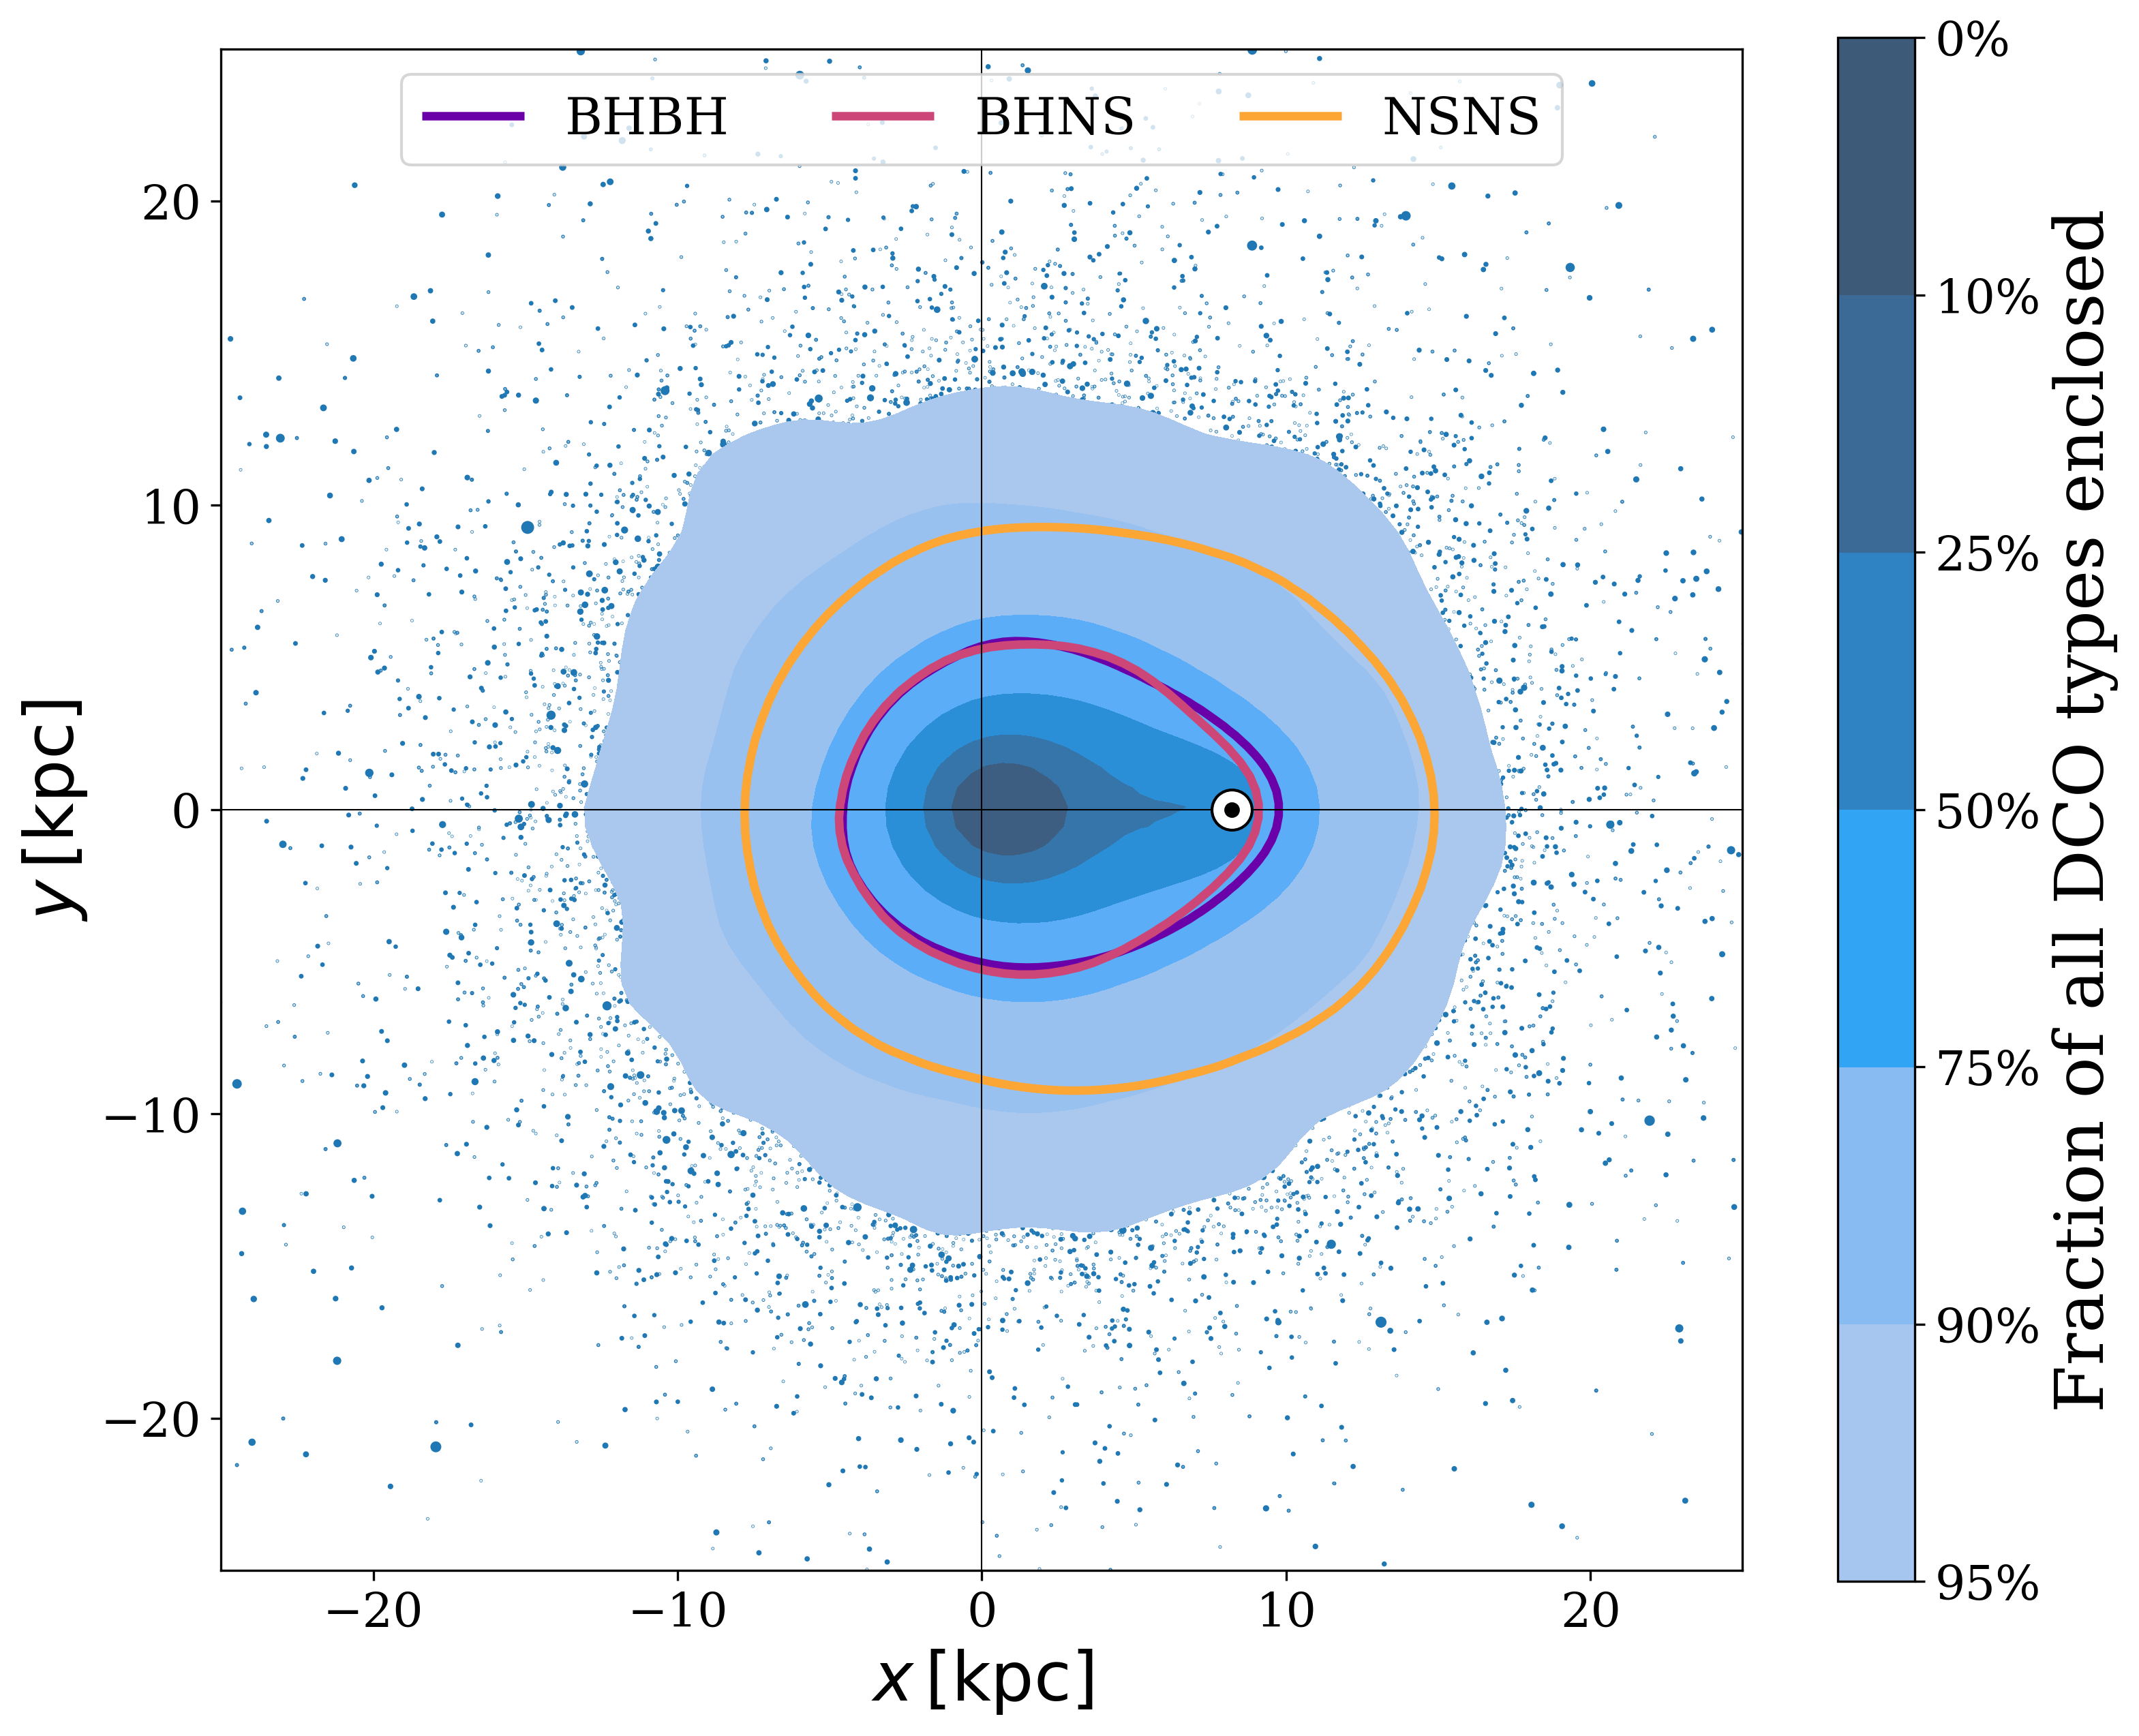
\includegraphics[width=\columnwidth]{fig4_1_galaxy_density_distribution.png}
    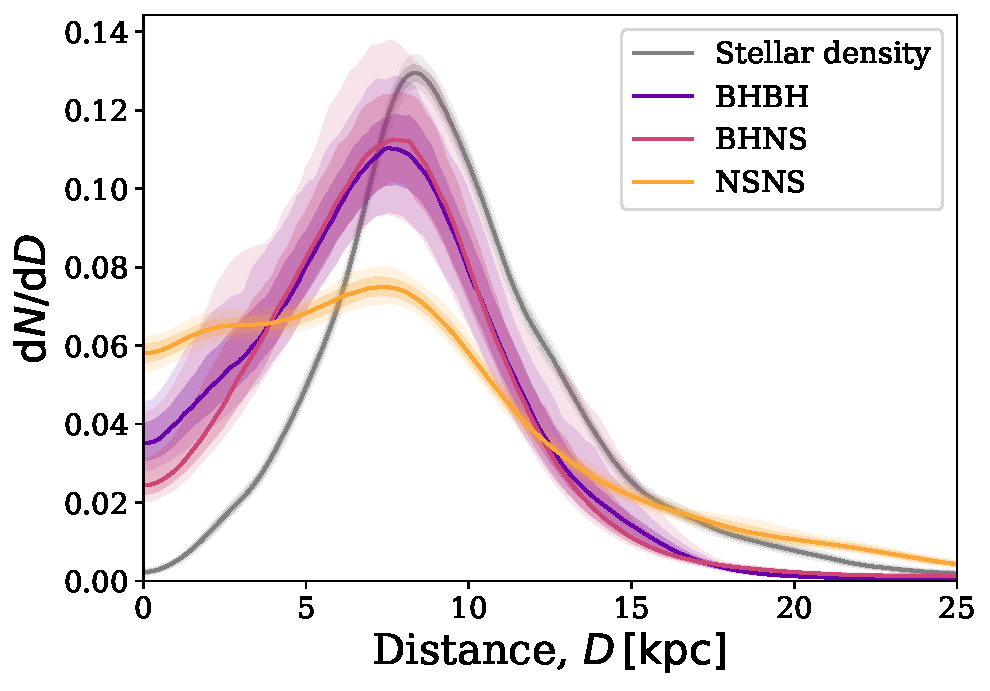
\includegraphics[width=\columnwidth]{fig4_2_detectable_distance_distribution_4yr.pdf}
    \caption{
    \textbf{Top:} A face-on view of the Galactic density distribution for detectable DCOs. We show the density distribution for the top 95\% of the sources, the rest are indicated by scatter points whose sizes correspond to their sampling weights. The coloured lines show the 75\% contour for each of the individual DCO types. The large cross passes through (0, 0) and helps to highlight the bias towards the position of the sun, which is indicated by the $\odot$.
    \textbf{Bottom:} As Fig.~\ref{fig:fiducial_pdf_distributions}, but for the luminosity distance. \href{https://github.com/TomWagg/detecting-DCOs-in-LISA/blob/main/paper/figures/fig4_1_galaxy_density_distribution.png}{\faFileImage} \href{https://github.com/TomWagg/detecting-DCOs-in-LISA/blob/main/paper/figure_notebooks/galaxy_creation_station.ipynb}{\faBook} \href{https://github.com/TomWagg/detecting-DCOs-in-LISA/blob/main/paper/figures/fig4_2_detectable_distance_distribution_4yr.pdf}{\faFileImage} \href{https://github.com/TomWagg/detecting-DCOs-in-LISA/blob/main/paper/figure_notebooks/fiducial.ipynb}{\faBook}.}
    \label{fig:detectable_distance_dist}
\end{figure}

In the top panel of Fig.~\ref{fig:detectable_distance_dist}, we show the density distribution for detectable DCOs in the galaxy. We see that most detectable sources are concentrated towards the Galactic centre, with a strong bias towards sources that are on our side of the Milky Way in the vicinity of the solar system (indicated with the $\odot$ symbol). In principle, systems are detectable out to large distances of about $20\unit{kpc}$ and more, although they become increasingly rare, as can be seen from the 95\% contour. 

The differences between different DCO types can be seen more clearly in the bottom panel of Fig.~\ref{fig:detectable_distance_dist} where we show the distribution of the distances, $D$, from earth to the detectable systems. Each distribution peaks around $8\unit{kpc}$, which is the distance to the centre of the Milky Way. The distribution for BHBH and BHNS systems follow a very similar shape, favouring the detection of systems with distance $<8\unit{kpc}$, but with a tail extending out to about $20\unit{kpc}$.

The distribution for NSNS stands out by being flatter, making them more common nearby and, surprisingly, also at larger distances compared to the stellar density. This may seem counter intuitive as one might naively expect the less massive NSNS systems would not be observable out to larger distances than the more massive BHNS and NSNS systems. To understand the differences we need to consider not only the mass distribution of binaries, but also their eccentricity and frequency distributions. Since, each parameter contributes to the calculation of the SNR (and thus affects the maximum distance at which systems can be detected).

The reason that the NSNSs are favoured at higher distances is that the NSNS population has the highest fraction of ``mildly'' eccentric systems ($0.01 < e < 0.03$). In contrast, the BHNS population has a much higher fraction of effectively circular systems ($e < 0.01$), which emit weaker gravitational waves compared to equivalent eccentric systems. Therefore, despite their typically higher masses, the distance at which a BHNS source is detectable is generally lower than for the mildly eccentric NSNS.

Conversely, the BHBH population has the highest fraction of highly eccentric systems ($e > 0.3$). Although one may naively expect that this would result in stronger signals (and so further distances), for a system to have these high eccentricities in LISA, it must still be early in its evolution (otherwise it would have circularised) and thus have a low orbital frequency. The result of this is that highest eccentricity systems tend to have lower SNRs and so cannot be detected at large distances. 

Overall we see that the eccentricity distribution of NSNSs occupies a ``sweet spot'' where the gravitational wave power is increased compared to circular systems, but it isn't too high that the frequency is significantly impacted. This means that NSNSs can be seen out to the largest distances of the three DCO types.

\subsection{Formation channels}\label{sec:progenitors_and_formation}
In our fiducial model, approximately two thirds of detectable BHBHs are formed through the `only stable mass transfer' channel, whilst the remaining third are primarily formed through the `classic' CE channel. Detectable BHNSs follow an inverse pattern, such that around two thirds are formed through the classic channel and the rest are mainly formed through only stable mass transfer.

In contrast, detectable NSNSs are very rarely formed through only stable mass transfer. Approximately half of systems are formed through the `classic' channel and the rest are formed through a double-core common-envelope event \citep{Brown+1995} where both progenitors evolve on a similar timescale and initiate a double-core common-envelope event whilst they are on the giant branch. All detectable DCOs show a small fraction of systems are formed through a channel that does not fit into the other categories and hence are labelled `other'. These systems tend to be formed through `lucky' supernova kicks that happen to shrink the binary significantly by chance.

The fraction of detectable DCOs that are formed through different formation channels in the other model variations are shown Fig.~\ref{fig:formation_channels}, where the first column in the plot corresponds to the fiducial model that we described above.

\subsection{How accurately will we be able to infer the parameters of detected systems?}\label{sec:measurement_uncertainties}
So far we have discussed the properties of the all detectable sources. However, only for a subset of systems we expect to get high enough SNR to obtain accurate and useful measurements of these parameters. Below we discuss the expected SNR distribution and the typical uncertainties expected for the most relevant parameters, namely, the chirp mass and sky localisation.

\paragraph{Signal-to-noise ratio}

\begin{figure}[tb]
    \centering
    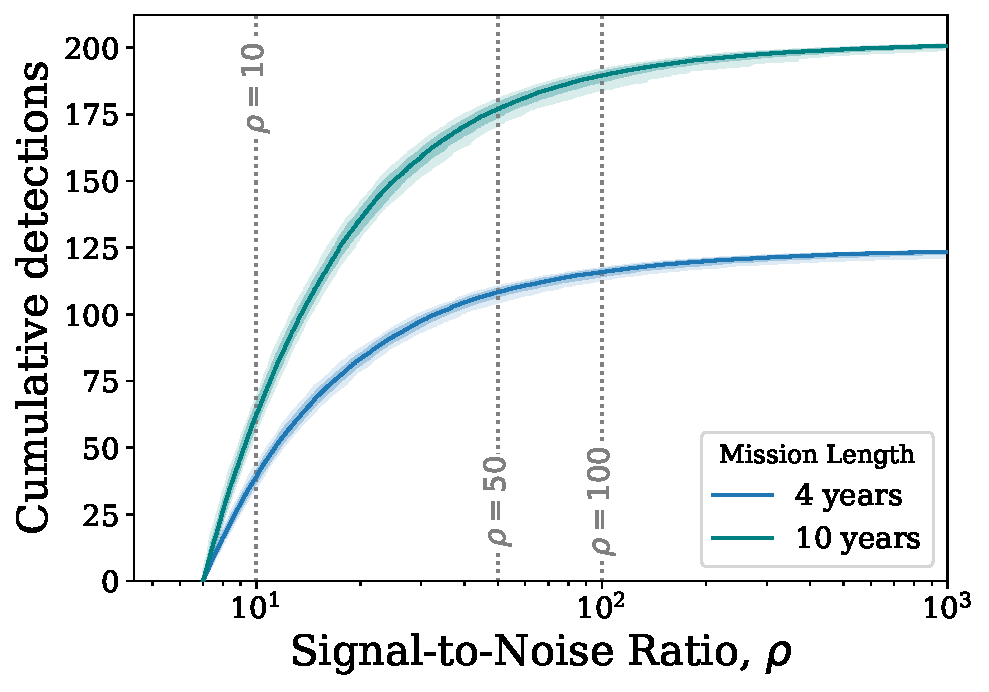
\includegraphics[width=\columnwidth]{fig5_snr_cumulative_all.pdf}
    \caption{Cumulative number of LISA detections with a given signal-to-noise ratio. Colours indicate LISA mission length and shading shows 1- and 2-$\sigma$ uncertainties (obtained via bootstrapping). \href{https://github.com/TomWagg/detecting-DCOs-in-LISA/blob/main/paper/figures/fig5_snr_cumulative_all.pdf}{\faFileImage} \href{https://github.com/TomWagg/detecting-DCOs-in-LISA/blob/main/paper/figure_notebooks/fiducial.ipynb}{\faBook}.}
    \label{fig:snr_dist}
\end{figure}

In Fig.~\ref{fig:snr_dist} we show the cumulative number of detections with a given SNR. Although many a large fraction of sources have SNRs around our assumed detection threshold of 7, many systems are detected with very high SNRs. We find that on average for a 4(10)-year LISA mission, of the 124(202) detections, 85(138), 16(27) and 9(14) systems have SNRs greater than 10, 50 and 100, respectively. These high SNR systems are typically, but not only, the more massive BHBH systems.

\paragraph{Chirp mass}

The chirp mass is important for identifying the type of the source of a detected GW signal. The uncertainty of the chirp mass depends on the uncertainty in the measured orbital frequency, the time derivative of the orbital frequency and the eccentricity as detailed in Appendix~\ref{app:chirp_mass_uncertainty}.

We find that for a 4(10)-year LISA mission, approximately 41(105) detections have measurable chirp masses ($\Delta \mathcal{M}_c / \mathcal{M}_c < 1$, indicated by the dark shaded region in Fig.~\ref{fig:m_c_unc}) whilst 13(31) have chirp mass uncertainties below 10\% ($\Delta \mathcal{M}_c / \mathcal{M}_c < 0.1$, indicated by the light shaded region in Fig.~\ref{fig:m_c_unc}). This uncertainty is generally dominated by the uncertainty on the time derivative of the frequency, since most of the binaries are too early in their inspiral for LISA to measure a strong chirp.
%
Note from Fig.~\ref{fig:m_c_unc} that increasing the mission length significantly increases the number of detections for which the chirp mass uncertainty is below 100\%. The total number of detections only scales as $\sqrt{T_{\rm obs}}$, yet we find that the the total number of detections with a chirp mass uncertainty is below 100\% and 10\% both scale approximately as $T_{\rm obs}$.

\begin{figure}[tb]
    \centering
    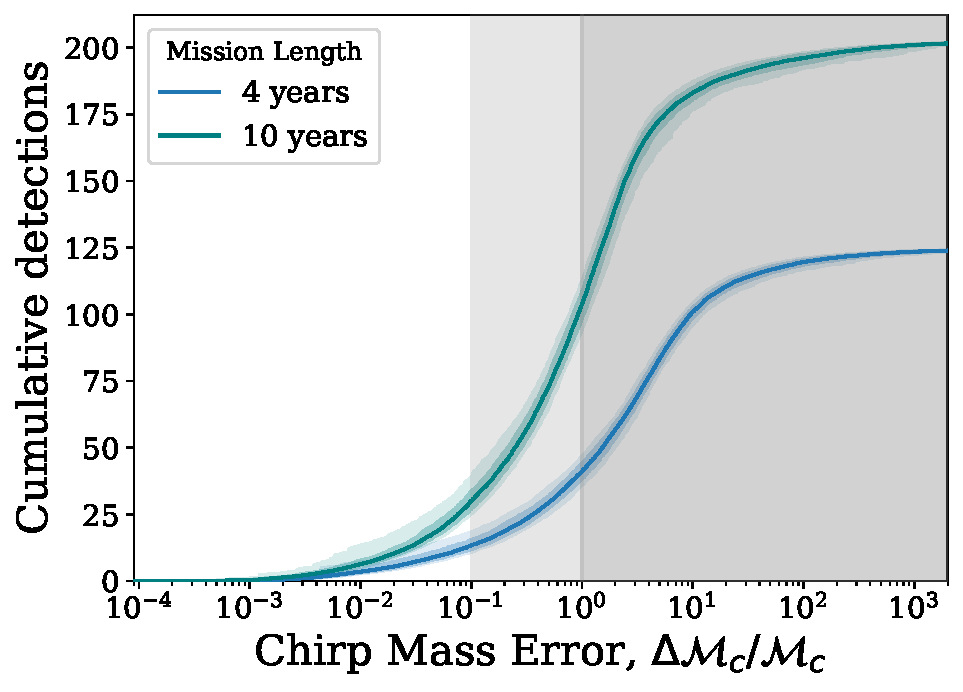
\includegraphics[width=\columnwidth]{fig6_chirp_mass_uncertainty_all.pdf}
    \caption{As Fig.~\ref{fig:snr_dist}, but for the chirp mass uncertainty. The shaded areas indicate regions with more than 10\% and 100\% uncertainty. \href{https://github.com/TomWagg/detecting-DCOs-in-LISA/blob/main/paper/figures/fig6_chirp_mass_uncertainty_all.pdf}{\faFileImage} \href{https://github.com/TomWagg/detecting-DCOs-in-LISA/blob/main/paper/figure_notebooks/fiducial.ipynb}{\faBook}.}
    \label{fig:m_c_unc}
\end{figure}

\paragraph{Sky localisation}

An accurate sky localisation will be essential to possibly identify electromagnetic counterparts or distinguish sources that come from different components of our Milky Way. 

We quantify the sky localisation of a source by estimating the angular resolution for the detectable sources. Since all potential sources are effectively stationary on the timescale of the LISA mission, we can follow \citet{Mandel+2018} and use the timing accuracy of LISA and the effective detector baseline to calculate the angular resolution, $\sigma_{\theta}$, as
\begin{equation}
    \sigma_{\theta} = 16.6^\circ \left(\frac{7}{\rho}\right) \left(\frac{5 \times 10^{-4} \unit{Hz}}{f_{\rm dom}}\right) \left( \frac{2 \unit{AU}}{L} \right),
\end{equation}
where $L$ is the effective detector baseline, which for LISA is 2 AU in the frame of the solar system, since it will orbit the Sun.

We plot the distribution of expected angular resolutions in Fig.~\ref{fig:ang_res}. We see that, for a 4(10)-year LISA mission, approximately 82(123) sources can be resolved to an angular resolution better than 10 degrees and only 16(23) better than 1 degree. 

For comparison, the size of a pencil beam for a $15 \unit{m}$ diameter SKA dish observing at 1.4 GHz is roughly 0.67 square degrees \citep{Smits+2009}, corresponding to an angular resolution of $\sigma_\theta = \sqrt{(0.67 / \pi)} = 0.46^\circ$ (similar to the angular size of the moon). We will further discuss the prospects of matching LISA detections to radio pulsars with SKA in Sec.~\ref{sec:pulsar_matching}.

\begin{figure}[htb]
    \centering
    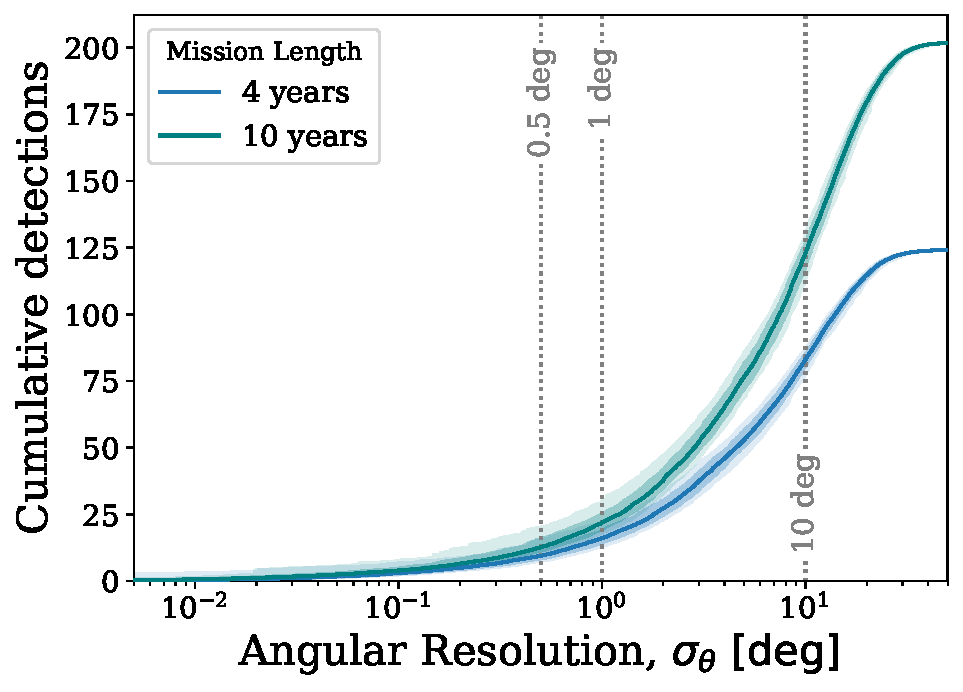
\includegraphics[width=\columnwidth]{fig7_angular_resolution_all.pdf}
    \caption{As Fig.~\ref{fig:snr_dist}, but for the angular resolution. \href{https://github.com/TomWagg/detecting-DCOs-in-LISA/blob/main/paper/figures/fig7_angular_resolution_all.pdf}{\faFileImage} \href{https://github.com/TomWagg/detecting-DCOs-in-LISA/blob/main/paper/figure_notebooks/fiducial.ipynb}{\faBook}.}
    \label{fig:ang_res}
\end{figure}